\documentclass[11pt,a4paper]{article}

% Datos de la actividad
\newcommand{\codigoactividad}{FORM-AC-01}
\newcommand{\nombreactividad}{Análisis de caso: fallo real en un sistema distribuido}
\newcommand{\caso}{GitHub, 21 de octubre de 2018}
\newcommand{\integrantes}{Castro Coello Mario Sebastián \\ Loor Suárez Steffanny del Rocío \\ Quintero Rico Luis David \\ Rivas Piloso Dayver Yahir}
\newcommand{\repositorio}{https://github.com/reyshadow0/isr701-form-ac-01}
\newcommand{\fechaentrega}{11 de noviembre de 2026}

\usepackage[T1]{fontenc}
\usepackage[utf8]{inputenc}
\usepackage[spanish,es-tabla,es-nodecimaldot]{babel}
\usepackage{lmodern}
\usepackage{microtype}
\usepackage[a4paper,margin=2.5cm]{geometry}
\usepackage{graphicx}
\usepackage{booktabs}
\usepackage{tabularx}
\usepackage{array}
\usepackage{float}
\usepackage{xcolor}
\usepackage{csquotes}
\usepackage[backend=biber,style=ieee]{biblatex}
\addbibresource{referencias.bib}
\usepackage[hidelinks]{hyperref}

\graphicspath{{diagrama/}}

% Permite cortar URL largas en la bibliografía (evita desbordes)
\setcounter{biburlnumpenalty}{100}
\setcounter{biburlucpenalty}{100}
\setcounter{biburllcpenalty}{100}

% Columna de ancho flexible con texto alineado a la izquierda
\newcolumntype{L}{>{\raggedright\arraybackslash}X}

\hypersetup{pdftitle={\codigoactividad: \nombreactividad}}

\begin{document}

\begin{titlepage}
  \centering
  {\large\bfseries UNIVERSIDAD TÉCNICA ESTATAL DE QUEVEDO\par}
  \vspace{0.3cm}
  {Facultad de Ciencias de la Computación\par}
  {Carrera de Software\par}
  \vspace{2.5cm}
  {\large Aplicaciones Distribuidas (ISR-701)\par}
  \vspace{1.5cm}
  {\Large\bfseries \codigoactividad\par}
  \vspace{0.4cm}
  {\LARGE \nombreactividad\par}
  \vspace{1cm}
  {\large Caso analizado: \caso\par}
  \vfill
  \begin{tabular}{@{}rl@{}}
    \textbf{Integrantes:}      & \begin{tabular}[t]{@{}l@{}}\integrantes\end{tabular} \\[2pt]
    \textbf{Docente:}          & Gleiston Cicerón Guerrero Ulloa, PhD \\
    \textbf{Nivel / paralelo:} & Séptimo nivel / B \\
    \textbf{Periodo:}          & SPA 2026--2027 \\
    \textbf{Fecha:}            & \fechaentrega \\
  \end{tabular}
  \par\vspace{1cm}
  {\small Repositorio: \url{\repositorio}\par}
\end{titlepage}

% Análisis: máximo 2 páginas (sin contar carátula ni referencias)
\section{Descripción del incidente}
\label{sec:incidente}
El incidente afectó a GitHub.com, cuyos servicios corrían en su mayoría en centros de datos propios. Sus metadatos se guardaban en clústeres MySQL con un primario para escrituras y réplicas para lecturas, y Orchestrator administraba la topología y el failover automático. Ocurrió entre el 21 y el 22 de octubre de 2018. Lo desencadenó un corte breve de conectividad entre el hub de red y el centro de datos principal de la Costa Este de Estados Unidos, durante el reemplazo de un equipo óptico que estaba fallando \cite{Warner2018}.
\begin{table}[H]
  \centering
  \small
  \caption{Línea de tiempo del incidente}
  \label{tab:linea-tiempo}
  \begin{tabularx}{\textwidth}{@{}p{3cm}L@{}}
    \toprule
    \textbf{Hora (UTC)} & \textbf{Evento} \\
    \midrule
21/10 22:52 & Se corta por unos segundos la conexión entre el hub de red y el centro de datos principal de la Costa Este, y Orchestrator pasa los primarios a la Costa Oeste. \\
21/10 22:54 & El monitoreo interno lanza alertas y varios ingenieros comienzan a revisarlas. \\
21/10 23:09 & GitHub pone el sitio en estado amarillo y poco después lo pasa a rojo. \\
21/10 23:19 & Se pausan los webhooks y las compilaciones de GitHub Pages para proteger los datos ya recibidos. \\
22/10 00:41 & Ya está en marcha la restauración desde backups de los clústeres afectados. \\
22/10 11:12 & Todos los primarios vuelven a la Costa Este, aunque decenas de réplicas siguen con horas de atraso. \\
22/10 16:24 & Con las réplicas sincronizadas se vuelve a la topología original, pero el estado sigue en rojo mientras se procesa lo acumulado. \\
22/10 23:03 & Se termina de procesar lo pendiente y el estado vuelve a verde. \\
    \bottomrule
  \end{tabularx}
\end{table}

\section{Causas raíz}
    \label{fig:causas}
El incidente comenzó con una interrupción de conectividad de 43 segundos \cite{Warner2018}
entre dos instalaciones de GitHub en la costa este de Estados Unidos. Esta desconexión momentánea provocó 
que Orchestrator promoviera réplicas de MySQL ubicadas en la costa oeste, aunque todavía existían escrituras que estaban 
pendientes de replicación, lo cual dio como resultado que las bases de datos quedaran en estados diferentes entre ambas regiones \cite{Warner2018}.
La recuperación fue complicada porque la nueva topología de MySQL no era compatible y generaba latencia entre regiones. Además, fue necesario restaurar respaldos, sincronizar réplicas y procesar trabajos acumulados. 
Estas condiciones prolongaron la degradación del servicio \cite{Warner2018}.
\begin{figure}[H]
    \centering
    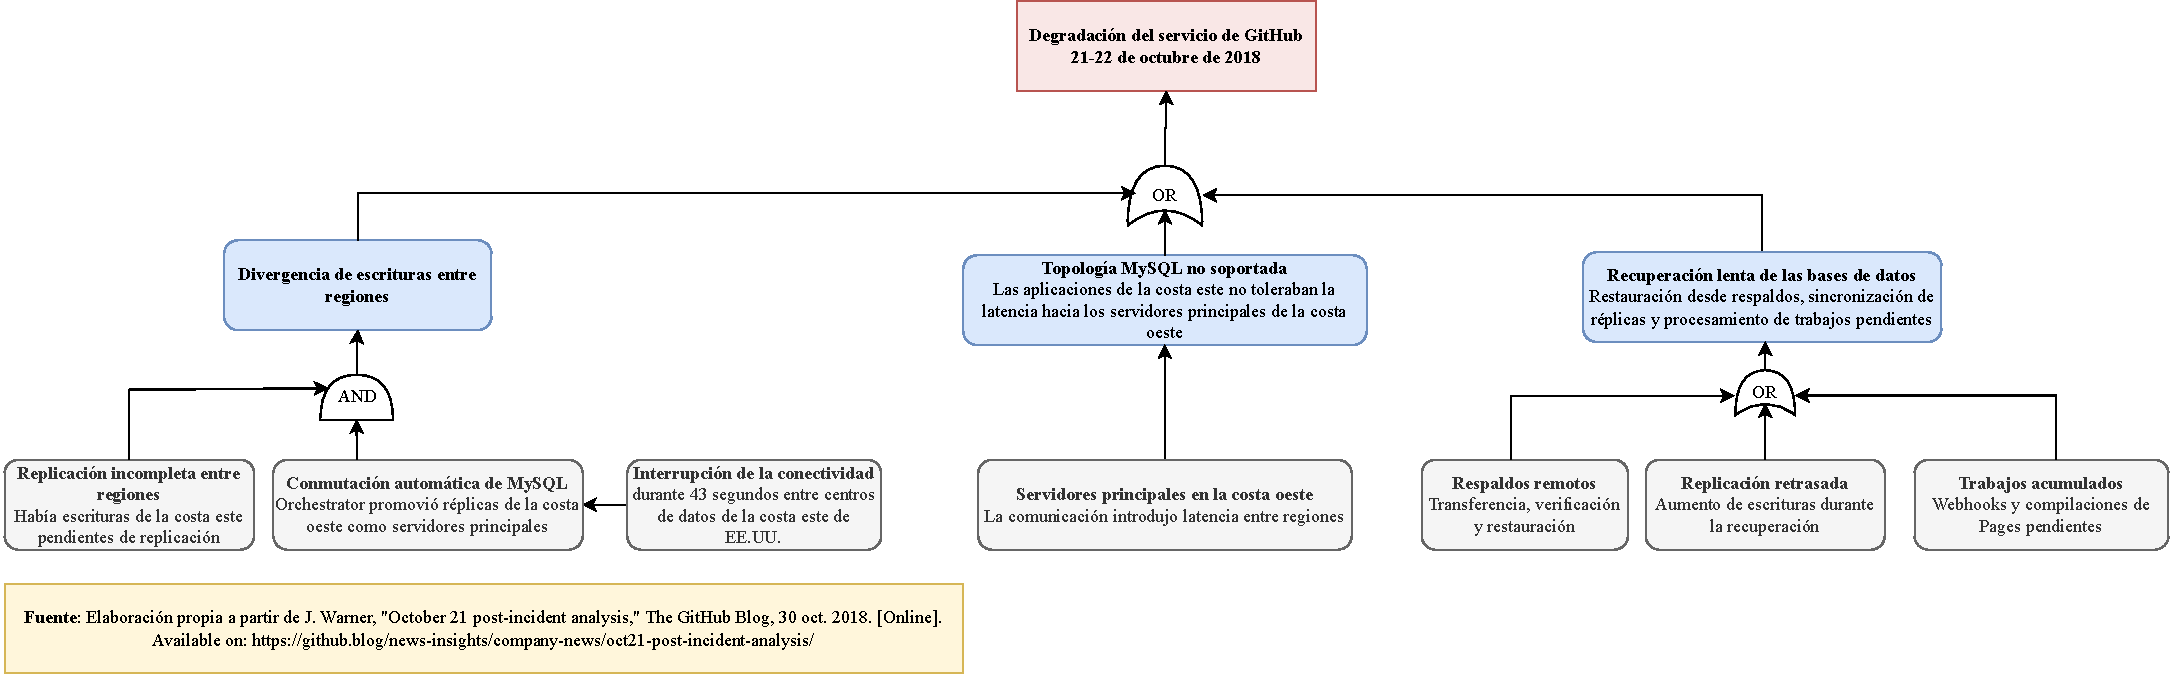
\includegraphics[width=\textwidth]{causas.pdf}
    \caption{Árbol de fallos del incidente de GitHub de octubre de 2018. Elaboración propia a partir de \cite{Warner2018}.}
\end{figure}
\section{Impacto}
\label{sec:impacto}

\section{Relación con la Unidad 1}
\label{sec:unidad1}

\subsection{Transparencia}

\subsection{Teorema CAP}

\subsection{Tolerancia a fallos}

\section{Mitigación de la empresa}
\label{sec:mitigacion}

\subsection{Inmediata}

\subsection{Permanente}

\section{Lecciones para el proyecto propio}
\label{sec:lecciones}

\begin{table}[H]
  \centering
  \small
  \caption{Riesgos del proyecto y medidas preventivas}
  \label{tab:riesgos}
  \begin{tabularx}{\textwidth}{@{}p{0.6cm}LL@{}}
    \toprule
    \textbf{N.\textdegree} & \textbf{Riesgo concreto} & \textbf{Medida preventiva} \\
    \midrule
    1 & & \\
    2 & & \\
    3 & & \\
    \bottomrule
  \end{tabularx}
\end{table}


\clearpage
\section{Retroalimentación recibida}
\label{sec:retroalimentacion}

\begin{table}[H]
  \centering
  \small
  \caption{Observaciones de pares y docente, y cómo se atendieron}
  \label{tab:retroalimentacion}
  \begin{tabularx}{\textwidth}{@{}p{2.4cm}LL@{}}
    \toprule
    \textbf{Quién} & \textbf{Observación} & \textbf{Cambio realizado o razón para no aplicarla} \\
    \midrule
     & & \\
    \bottomrule
  \end{tabularx}
\end{table}

\section{Declaración de uso de inteligencia artificial}
\label{sec:declaracion-ia}

\begin{table}[H]
  \centering
  \small
  \caption{Herramientas de inteligencia artificial usadas como apoyo}
  \label{tab:declaracion-ia}
  \begin{tabularx}{\textwidth}{@{}p{2.5cm}p{1.7cm}LL@{}}
    \toprule
    \textbf{Herramienta} & \textbf{Versión} & \textbf{Para qué se usó} & \textbf{Cómo se verificó lo obtenido} \\
    \midrule
     & & & \\
    \bottomrule
  \end{tabularx}
\end{table}


\printbibliography[heading=bibintoc,title={Referencias}]

\end{document}
